%Chapter 4
\chapter{Research Findings}
\label{Chapter4}
\section{Run Results and Analysis Tools}
If the no free lunch theorem applies to  meta-learning strategies, we
should see near equal performance across a variety of meta-set collections.
We will call this assertion the null hypothesis, that is to say our null
hypothesis is that the meta-learning strategies used in this experiment
are equal.

In order to test the null hypothesis, 30 such samples of the kind described
in Chapter 3 were collected. The metrics of interest on these samples are
contained in the tables within this chapter. How often the algorithms placed
first, second, or third can be seen in table 4.1. The average of these
placements across all samples, i.e the algorithms average placements, can be
seen in table 4.2. Table 4.3 contains the proportion of probability for the
results contained in table 4.1. Table 4.4 contains the average of the
proportion of probabilities contained in table 4.3 across all samples.
Table 4.5 contains the standard deviations of the placement values for the
meta-algorithms. Table 4.6 contains the t scores of each of the values present
in table 4.1. Table 4.7 contains the average of the t scores contained in
table 4.6 across all samples and it is this table that I use later to draw the
conclusion that the null hypothesis may be safely rejected.

\begin{table}
\begin{tabular}{|l|rrr|rrr|rrr|}
\toprule

& \multicolumn{3}{c|} {GuessesActive}  & \multicolumn{3}{c|}{GuessesEx}  & \multicolumn{3}{c|}{GuessesSamp}  \\
\midrule
     &   First &  Second &  Third &         First &  Second  &  Third &           First &  Second &  Third \\
\midrule
sample 1   &             1 &  4 &  5 &         6 &  2 &  2 &           3 &  4 &  3 \\
sample 2   &             1 &  4 &  5 &         5 &  2 &  3 &           4 &  4 &  2 \\
sample 3   &             1 &  3 &  6 &         7 &  3 &  0 &           2 &  4 &  4 \\
sample 4   &             1 &  5 &  4 &         6 &  3 &  1 &           3 &  2 &  5 \\
sample 5   &             0 &  6 &  4 &         8 &  2 &  0 &           2 &  2 &  6 \\
sample 6   &             3 &  3 &  4 &         5 &  4 &  1 &           2 &  3 &  5 \\
sample 7   &             4 &  3 &  3 &         4 &  4 &  2 &           2 &  3 &  5 \\
sample 8   &             2 &  3 &  5 &         7 &  2 &  1 &           1 &  5 &  4 \\
sample 9   &             1 &  3 &  6 &         3 &  5 &  2 &           6 &  2 &  2 \\
sample 10  &             0 &  4 &  6 &         7 &  3 &  0 &           3 &  3 &  4 \\
sample 11  &             0 &  6 &  4 &         7 &  3 &  0 &           3 &  1 &  6 \\
sample 12 &             1 &  5 &  4 &         7 &  2 &  1 &           2 &  3 &  5 \\
sample 13 &             3 &  3 &  4 &         5 &  4 &  1 &           2 &  3 &  5 \\
sample 14 &             2 &  5 &  3 &         6 &  3 &  1 &           2 &  2 &  6 \\
sample 15 &             2 &  1 &  7 &         4 &  6 &  0 &           4 &  3 &  3 \\
sample 16 &             1 &  5 &  4 &         6 &  0 &  4 &           3 &  5 &  2 \\
sample 17 &             1 &  4 &  5 &         6 &  4 &  0 &           3 &  2 &  5 \\
sample 18 &             1 &  3 &  6 &         8 &  1 &  1 &           1 &  6 &  3 \\
sample 19 &             1 &  4 &  5 &         7 &  3 &  0 &           2 &  3 &  5 \\
sample 20 &             2 &  4 &  4 &         6 &  2 &  2 &           2 &  4 &  4 \\
sample 21 &             1 &  2 &  7 &         4 &  6 &  0 &           5 &  2 &  3 \\
sample 22 &             3 &  3 &  4 &         2 &  7 &  1 &           5 &  0 &  5 \\
sample 23 &             3 &  4 &  3 &         6 &  4 &  0 &           1 &  2 &  7 \\
sample 24 &             3 &  3 &  4 &         4 &  4 &  2 &           3 &  3 &  4 \\
sample 25 &             2 &  6 &  2 &         7 &  3 &  0 &           1 &  1 &  8 \\
sample 26 &             1 &  3 &  6 &         6 &  2 &  2 &           3 &  5 &  2 \\
sample 27 &             7 &  2 &  1 &         3 &  5 &  2 &           0 &  3 &  7 \\
sample 28 &             0 &  5 &  5 &         7 &  2 &  1 &           3 &  3 &  4 \\
sample 29 &             1 &  2 &  7 &         4 &  5 &  1 &           5 &  3 &  2 \\
sample 30 &             2 &  6 &  2 &         4 &  3 &  3 &           4 &  1 &  5 \\
\bottomrule
\end{tabular}
\caption{Placement results}
\end{table}


\begin{table}
\begin{tabular}{lrrr}
\toprule
{} &  GuessesActive &  GuessesEx &  GuessesSamp \\
\midrule
First  &           1.70 &        3.8 &         4.50 \\
Second &           5.57 &        3.3 &         1.13 \\
Third  &           2.73 &        2.9 &         4.37 \\
\bottomrule
\end{tabular}
\caption{Average placement results across all samples}
\end{table}

Each of the meta-set collections contains 10 basesets and the experiment
compares the performance of 3 meta-learning algorithms. As such, the expected
average number of first, second, and third place finishes given that the
meta-learning algorithms are equal is 3.3. The values seen within the placement
counts table given equal meta-learning algorithms should more often than not be
either 3 or 4 and the averages of the placements across all samples should all
be near 3.3. Instead, it appears that the sampler performed the best,
with an average number of first place finshes of 4.5. Moreover most of the
averages present in table 4.2 seem to be farther away from the expected value of
3.3 than one would intuitively expect if the meta-learning algorithms were
truly equal. Whether or not these results fall far enough outside
expectation in order to reject the null hypothesis requires analysis with the
machinary of classical statistics. Three well established hypothesis testing
measures are the method of calculating sampling distribution probabilities,
analysis of variance (anova) and t score analysis. A brief description of each
of these statistical methods and the result from their usage follows.

\subsection{Exact Sampling Distribution}
The following description losely follows the procedure described in \cite{Cohen}.
In it, the author asks the reader to imagine testing a coin to see whether or
not it is fair, flipping the coin 1,2,..N times. He then asks the reader to
consider whether some proportion of heads is actually fair from 0/N, 1/N.., N/N
heads. The propability that some proportion of heads p = i/N is fair can be
calculated exactly with the binomial distribution
$$\frac{N!}{i!(N-i)!}r^{i}(1-r)^{N-i}$$
This situation is analogous to the number of first, second, or third place
finishes some meta-algorithm obtained in this thesis experiment. The probabilty
of proportions for each of the meta-learning algorithms can be seen in table 4.3
and the average of these proportions across all samples can be seen in table 4.4.

\begin{table}
\begin{tabular}{|l|rrr|rrr|rrr|}
\toprule
& \multicolumn{3}{c|}{GuessesActive} & \multicolumn{3}{c|}{GuessesEx} & \multicolumn{3}{c|}{GuessesSamp} \\
\midrule
 &             First &     Second &     Third &   First &     Second &     Third &     First &     Second &  Third \\
\midrule
sample 1  &          0.09 &  0.23 &  0.14 &      0.06 &  0.20 &  0.20 &        0.26 &  0.23 &  0.26 \\
sample 2  &          0.09 &  0.23 &  0.14 &      0.14 &  0.20 &  0.26 &        0.23 &  0.23 &  0.20 \\
sample 3  &          0.09 &  0.26 &  0.06 &      0.02 &  0.26 &  0.02 &        0.20 &  0.23 &  0.23 \\
sample 4  &          0.09 &  0.14 &  0.23 &      0.06 &  0.26 &  0.09 &        0.26 &  0.20 &  0.14 \\
sample 5  &          0.02 &  0.06 &  0.23 &      0.00 &  0.20 &  0.02 &        0.20 &  0.20 &  0.06 \\
sample 6  &          0.26 &  0.26 &  0.23 &      0.14 &  0.23 &  0.09 &        0.20 &  0.26 &  0.14 \\
sample 7  &          0.23 &  0.26 &  0.26 &      0.23 &  0.23 &  0.20 &        0.20 &  0.26 &  0.14 \\
sample 8  &          0.20 &  0.26 &  0.14 &      0.02 &  0.20 &  0.09 &        0.09 &  0.14 &  0.23 \\
sample 9  &          0.09 &  0.26 &  0.06 &      0.26 &  0.14 &  0.20 &        0.06 &  0.20 &  0.20 \\
sample 10 &          0.02 &  0.23 &  0.06 &      0.02 &  0.26 &  0.02 &        0.26 &  0.26 &  0.23 \\
sample 11 &          0.02 &  0.06 &  0.23 &      0.02 &  0.26 &  0.02 &        0.26 &  0.09 &  0.06 \\
sample 12 &          0.09 &  0.14 &  0.23 &      0.02 &  0.20 &  0.09 &        0.20 &  0.26 &  0.14 \\
sample 13 &          0.26 &  0.26 &  0.23 &      0.14 &  0.23 &  0.09 &        0.20 &  0.26 &  0.14 \\
sample 14 &          0.20 &  0.14 &  0.26 &      0.06 &  0.26 &  0.09 &        0.20 &  0.20 &  0.06 \\
sample 15 &          0.20 &  0.09 &  0.02 &      0.23 &  0.06 &  0.02 &        0.23 &  0.26 &  0.26 \\
sample 16 &          0.09 &  0.14 &  0.23 &      0.06 &  0.02 &  0.23 &        0.26 &  0.14 &  0.20 \\
sample 17 &          0.09 &  0.23 &  0.14 &      0.06 &  0.23 &  0.02 &        0.26 &  0.20 &  0.14 \\
sample 18 &          0.09 &  0.26 &  0.06 &      0.00 &  0.09 &  0.09 &        0.09 &  0.06 &  0.26 \\
sample 19 &          0.09 &  0.23 &  0.14 &      0.02 &  0.26 &  0.02 &        0.20 &  0.26 &  0.14 \\
sample 20 &          0.20 &  0.23 &  0.23 &      0.06 &  0.20 &  0.20 &        0.20 &  0.23 &  0.23 \\
sample 21 &          0.09 &  0.20 &  0.02 &      0.23 &  0.06 &  0.02 &        0.14 &  0.20 &  0.26 \\
sample 22 &          0.26 &  0.26 &  0.23 &      0.20 &  0.02 &  0.09 &        0.14 &  0.02 &  0.14 \\
sample 23 &          0.26 &  0.23 &  0.26 &      0.06 &  0.23 &  0.02 &        0.09 &  0.20 &  0.02 \\
sample 24 &          0.26 &  0.26 &  0.23 &      0.23 &  0.23 &  0.20 &        0.26 &  0.26 &  0.23 \\
sample 25 &          0.20 &  0.06 &  0.20 &      0.02 &  0.26 &  0.02 &        0.09 &  0.09 &  0.00 \\
sample 26 &          0.09 &  0.26 &  0.06 &      0.06 &  0.20 &  0.20 &        0.26 &  0.14 &  0.20 \\
sample 27 &          0.02 &  0.20 &  0.09 &      0.26 &  0.14 &  0.20 &        0.02 &  0.26 &  0.02 \\
sample 28 &          0.02 &  0.14 &  0.14 &      0.02 &  0.20 &  0.09 &        0.26 &  0.26 &  0.23 \\
sample 29 &          0.09 &  0.20 &  0.02 &      0.23 &  0.14 &  0.09 &        0.14 &  0.26 &  0.20 \\
sample 30 &          0.20 &  0.06 &  0.20 &      0.23 &  0.26 &  0.26 &        0.23 &  0.09 &  0.14 \\
\bottomrule
\end{tabular}
\caption{Placement results proportion probabilities}
\end{table}


\begin{table}
\begin{tabular}{lrrr}
\toprule
{} &  GuessesActive &  GuessesEx &  GuessesSamp \\
\midrule
First  &        0.13 &       0.19 &         0.16 \\
Second &        0.10 &       0.19 &         0.11 \\
Third  &        0.19 &       0.20 &         0.16 \\
\bottomrule
\end{tabular}
\caption{Average of proportion probabilities across all samples}
\end{table}

We can calculate the probability of drawing either of the values closest
to expectation, 3 or 4, by use of the previously mentioned binomial distribution,
with $N = 10$, $r = 0.33$, and $i$ being either 3 or 4. The values we get for
the propabilities of the most expected values are then 0.26 and 0.22
respectively. The average of all values within this table is
0.15, significantly lower than the probability of the expected value.
Still, this is not enough to reject the null hypothesis as proportion
probability analysis does not come with a rejection criteria.

\subsection{Analysis of Variance}
Analysis of variance is a test that decomposes the variance in data and shows
how much of it is due to random variations and how much is due to the influence
of a factor \cite{Cohen}. It allows one to measure the probability that the means
of a group of distributions is the same. It is often used as an exploratory tool
to explain observations, and it is in this spirit that it is used here.

To perform anova, one requires the means of the groups under consideration, the
variance of the groups under consideration, the ``grand  mean'' of the groups
under consideration (the mean of each group mean), and the ``grand variance''
of the groups under consideration (the normalized sum of the variances of the
group). The grand mean and grand variance are then used to find the mean square
value of the deviations of the variances within and between the groups. The
test is then comprised of taking the ration between these values, with rejection
or acceptance of the null hypothesis (in the case of anova almost always that
the means are equal) then depending on how many ``degrees of freedom'' were
involved in the calculation of the mean squared values.

Inspecting the representative equations clarifies the procedure. Consider first,
the deviation of a value from its grand mean:

$$e_{j,k} = (x_{j,k} - \overline{x}_{G}),$$

where $x$ is an observed value, $e$ is its variance, $j$ is a groups label
and $k$ is the within group label of the given value. Taking the sum of the
squares of all of these across each of the groups gives us the sample grand
variance:

$$s_{G}^{2} = \frac{\sum{}_{j}\sum_{k}{(x_{j,k} - \overline{x}_{G})^{2}}}{N-1} = \frac{SS_{total}}{df_{total}},$$

where the total degrees of freedom $df$ is equal to the total number of items in
all the groups  $N$ minus the one way that the variances are not free to vary 1
(the grand variance itself). The total sum of squares $SS_{total}$ can be broken
up into two components: $SS_{total} = SS_{between} + SS_{within}$ where the sum
of squares between the groups is equal to:

$$SS_{between} = \sum_{j}n_{j}(\overline{x}_{j}-\overline{x}_{G})^{2},$$

and the sum of squares within the groups is equal to:

$$SS_{within} = \sum_{j}\sum_{k}(x_{j,k} - \overline{x}_{j})^{2}.$$

By taking the degrees of freedom between groups and within groups, we can obtain
the mean square deviations between and within the groups via division. The
degrees of freedom between the groups is equal to the number of groups $j$ minus 1
and the number of degrees of freedom within the groups is equal to the total
number of items $N$ minus the number of groups those items are contained within
$j$. The mean square deviations are then as follows:

$$MS_{between} = \frac{SS_{between}}{df_{between}} = \frac{\sum_{j}n_{j}(\overline{x}_{j}-\overline{x}_{G})^{2}}{j-1};$$

$$MS_{within} = \frac{SS_{within}}{df_{within}} = \frac{\sum_{j}\sum_{k}(x_{j,k}-\overline{x}_{j})^{2}}{N-j}.$$

The value then used to score the sample is the $F$ statistic

$$F = \frac{MS_{between}}{MS_{within}}.$$

Notice that $MS_{between}$ and $MS_{within}$ are variances - sums of squares
divided by degrees of freedom - so $F$ is a ratio of variances, and under $H_{0}$
(the null hypothesis) these variances are equal \cite{Cohen}. The distribution
with which on compares this results is the $F$ distribution and the values that
determine the critical point within this distribution are $j-1$ and $N-j$, which
are the degrees of freedom of the $F$ values numerator and denominator.

An analysis of variance of the results of this experiment was conducted by passing
the results into an excel spread sheet then running excels native anova tool on
the items. The results where as follows:

\begin{figure}[h]
\resizebox{\columnwidth}{!}{%
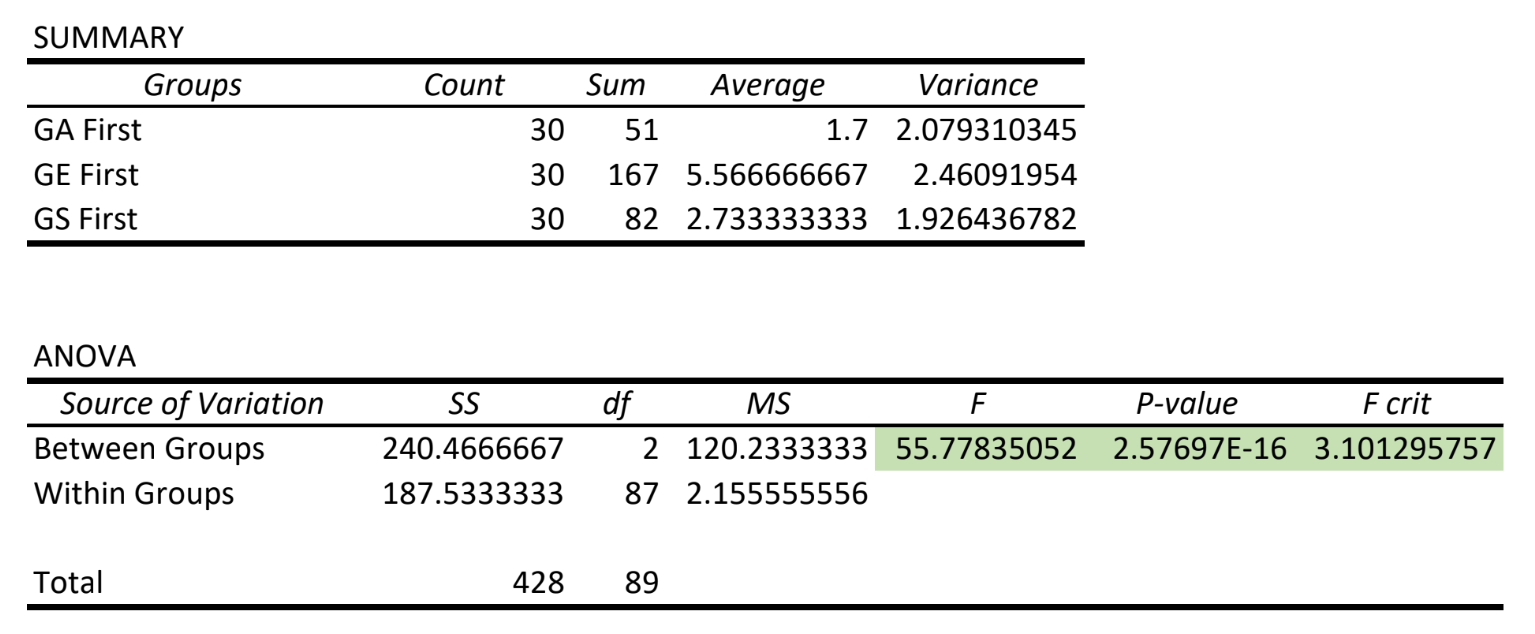
\includegraphics{Chapters/Images/ANOVA/ANOVAFirst.PNG}
}
\caption{ANOVA analysis of first placements}
\end{figure}

\begin{figure}[h]
\resizebox{\columnwidth}{!}{%
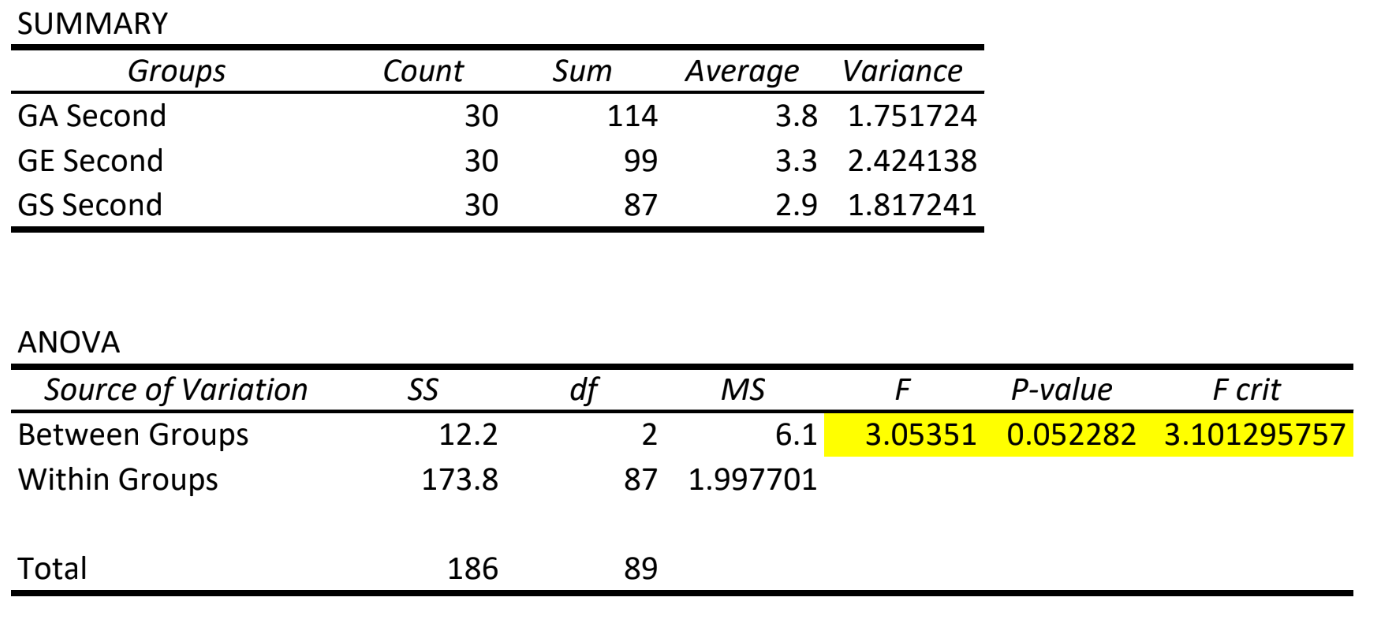
\includegraphics{Chapters/Images/ANOVA/ANOVASecond.PNG}
}
\caption{ANOVA analysis of second placements}
\end{figure}

\begin{figure}[h]
\resizebox{\columnwidth}{!}{%
\includegraphics{Chapters/Images/ANOVA/ANOVAThird.PNG}
}
\caption{ANOVA analysis of third placements}
\end{figure}

The probability of the ``F'' values of the first and second placement columns is
increadibly low, leading one to suspect that we can reject the null hypothesis.
This suspicion will be confirmed in formalized in the next section after we
apply the $t$ test.

\subsection{$t$ score}
$t$ score analysis is a form of hypothesis testing that allows one to determine
whether or not some result emerged from some given distribution via consideration
of how many standard deviations the result deviates from the mean of said given
distribution. Its equation has the form:
$$t =\frac{\overline{x}-\mu}{\hat{\sigma}_{\overline{x}}} = \frac{\overline{x}-\mu}{\frac{s}{\sqrt{N}}}$$
where $s$ is the sample standard deviation, $N$ is the number of samples,
$\overline{x}$ is an individual samples mean/calculated value, and $\mu$ is
the mean of the distribution of comparison.

The decision as to whether or not a specific $t$ score value implies a result
is from a different distribution depends on how many samples were used in the
calculation of the sample mean and on what the desired confidence interval is.
The critical threshold used in order to make this decision is gained by the use
of $t$ distribution table. In the case where 30 samples are used and the desired
margin of error is 5\%, the critical thresholds for a two tailed $t$ test are
-2.042 and 2.042. If the averaged values of the $t$ scores falls outside of
these bounds then we can reject the null hypothesis with a 5 \% margin of error.
The standard deviations for each of the samples can be seen in table 4.5. Taking
these with the average placement results available in table 4.2 allows the
calculating of the desired $t$ scores, which can be seen in table 4.6. Taking
the average of the absolute value of each of these $t$ scores
yeilds 5.11. We can thus comfortably reject the null hypothesis.


\begin{table}
\begin{tabular}{lrrr}
\toprule
{} &  GuessesActive &  GuessesEx &  GuessesSamp \\
\midrule
First  &           1.42 &       1.30 &     1.48 \\
Second &           1.54 &       1.53 &     1.06 \\
Third  &           1.36 &       1.33 &     1.58 \\
\bottomrule
\end{tabular}
\caption{Placement results standard deviations across all samples}
\end{table}


%% \begin{table}
%% \begin{tabular}{lrrrrrrrrr}
%% \toprule
%% algorithms & \multicolumn{3}{l}{GuessesActive} & \multicolumn{3}{l}{GuessesEx} & \multicolumn{3}{l}{GuessesSamp} \\
%% positions &  First &   Second &    Third &    First &  Second &  Third &    First &  Second &  Third \\
%% \midrule
%% sample 1  &        -10.41 &   3.24 &   7.13 &     10.93 &  -5.51 &  -7.98 &       -1.54 &   3.18 &  -1.33 \\
%% sample 2  &        -10.41 &   3.24 &   7.13 &      6.83 &  -5.51 &  -2.00 &        3.09 &   3.18 &  -5.33 \\
%% sample 3  &        -10.41 &  -1.62 &  11.41 &     15.04 &  -1.38 & -19.96 &       -6.18 &   3.18 &   2.67 \\
%% sample 4  &        -10.41 &   8.10 &   2.85 &     10.93 &  -1.38 & -13.97 &       -1.54 &  -6.36 &   6.67 \\
%% sample 5  &        -14.87 &  12.96 &   2.85 &     19.14 &  -5.51 & -19.96 &       -6.18 &  -6.36 &  10.67 \\
%% sample 6  &         -1.49 &  -1.62 &   2.85 &      6.83 &   2.75 & -13.97 &       -6.18 &  -1.59 &   6.67 \\
%% sample 7  &          2.97 &  -1.62 &  -1.43 &      2.73 &   2.75 &  -7.98 &       -6.18 &  -1.59 &   6.67 \\
%% sample 8  &         -5.95 &  -1.62 &   7.13 &     15.04 &  -5.51 & -13.97 &      -10.81 &   7.95 &   2.67 \\
%% sample 9  &        -10.41 &  -1.62 &  11.41 &     -1.37 &   6.89 &  -7.98 &       12.36 &  -6.36 &  -5.33 \\
%% sample 10 &        -14.87 &   3.24 &  11.41 &     15.04 &  -1.38 & -19.96 &       -1.54 &  -1.59 &   2.67 \\
%% sample 11 &        -14.87 &  12.96 &   2.85 &     15.04 &  -1.38 & -19.96 &       -1.54 & -11.13 &  10.67 \\
%% sample 12 &        -10.41 &   8.10 &   2.85 &     15.04 &  -5.51 & -13.97 &       -6.18 &  -1.59 &   6.67 \\
%% sample 13 &         -1.49 &  -1.62 &   2.85 &      6.83 &   2.75 & -13.97 &       -6.18 &  -1.59 &   6.67 \\
%% sample 14 &         -5.95 &   8.10 &  -1.43 &     10.93 &  -1.38 & -13.97 &       -6.18 &  -6.36 &  10.67 \\
%% sample 15 &         -5.95 & -11.34 &  15.69 &      2.73 &  11.02 & -19.96 &        3.09 &  -1.59 &  -1.33 \\
%% sample 16 &        -10.41 &   8.10 &   2.85 &     10.93 & -13.77 &   3.99 &       -1.54 &   7.95 &  -5.33 \\
%% sample 17 &        -10.41 &   3.24 &   7.13 &     10.93 &   2.75 & -19.96 &       -1.54 &  -6.36 &   6.67 \\
%% sample 18 &        -10.41 &  -1.62 &  11.41 &     19.14 &  -9.64 & -13.97 &      -10.81 &  12.72 &  -1.33 \\
%% sample 19 &        -10.41 &   3.24 &   7.13 &     15.04 &  -1.38 & -19.96 &       -6.18 &  -1.59 &   6.67 \\
%% sample 20 &         -5.95 &   3.24 &   2.85 &     10.93 &  -5.51 &  -7.98 &       -6.18 &   3.18 &   2.67 \\
%% sample 21 &        -10.41 &  -6.48 &  15.69 &      2.73 &  11.02 & -19.96 &        7.72 &  -6.36 &  -1.33 \\
%% sample 22 &         -1.49 &  -1.62 &   2.85 &     -5.47 &  15.15 & -13.97 &        7.72 & -15.91 &   6.67 \\
%% sample 23 &         -1.49 &   3.24 &  -1.43 &     10.93 &   2.75 & -19.96 &      -10.81 &  -6.36 &  14.67 \\
%% sample 24 &         -1.49 &  -1.62 &   2.85 &      2.73 &   2.75 &  -7.98 &       -1.54 &  -1.59 &   2.67 \\
%% sample 25 &         -5.95 &  12.96 &  -5.71 &     15.04 &  -1.38 & -19.96 &      -10.81 & -11.13 &  18.67 \\
%% sample 26 &        -10.41 &  -1.62 &  11.41 &     10.93 &  -5.51 &  -7.98 &       -1.54 &   7.95 &  -5.33 \\
%% sample 27 &         16.36 &  -6.48 &  -9.99 &     -1.37 &   6.89 &  -7.98 &      -15.45 &  -1.59 &  14.67 \\
%% sample 28 &        -14.87 &   8.10 &   7.13 &     15.04 &  -5.51 & -13.97 &       -1.54 &  -1.59 &   2.67 \\
%% sample 29 &        -10.41 &  -6.48 &  15.69 &      2.73 &   6.89 & -13.97 &        7.72 &  -1.59 &  -5.33 \\
%% sample 30 &         -5.95 &  12.96 &  -5.71 &      2.73 &  -1.38 &  -2.00 &        3.09 & -11.13 &   6.67 \\
%% \bottomrule
%% \end{tabular}
%% \caption{Placement results t scores}
%% \end{table}

\begin{table}
\begin{tabular}{lrrr}
\toprule
{} &  GuessesActive &  GuessesEx &  GuessesSamp \\
\midrule
First  &      -6.29 &       1.98 &         4.32 \\
Second &       7.97 &      -0.11 &       -11.36 \\
Third  &      -2.42 &      -1.77 &         3.61 \\
\bottomrule
\end{tabular}
\caption{t scores of placement averages}
\end{table}
